\chapter{Constraint solvers}
\thispagestyle{myheadings}\markright{$ $Id$ $}

In this chapter we will describe various CSP solvers. We will focus on the specific
properties of each solver. All described solvers support most of constraints listed 
in table \ref{table-basic-constraints} (we will call them basic constraints).

\begin{table}
\caption{\label{}Basic constraints supported by all tested solvers}
\begin{center}
\begin{tabular}{|l|p{4cm}|}
\hline \verb=alldifferent([=$q_0, q_1, \dots$\verb=])= &  $\forall i,j: j \neq i \Rightarrow q_i \neq q_i$ \\
\hline \verb=eq(=$a$\verb=,= $b$\verb=)= &  $a = b$ \\
\hline \verb=neq(=$a$\verb=,= $b$\verb=)= &  $a \neq b$ \\
\hline \verb=abs(=$a$\verb=,= $b$\verb=)= &  $a = |b|$ \\
\hline \verb=lt(=$a$\verb=,= $b$\verb=)= &  $a < b$ \\
\hline \verb=gt(=$a$\verb=,= $b$\verb=)= &  $a > b$ \\
\hline \verb=leq(=$a$\verb=,= $b$\verb=)= &  $a \leq b$ \\
\hline \verb=geq(=$a$\verb=,= $b$\verb=)= &  $a \geq b$ \\
\hline \verb=plus(=$a$\verb=,= $b$\verb=,= $c$\verb=)= &  $a + b = c$ \\
\hline \verb=minus(=$a$\verb=,= $b$\verb=,= $c$\verb=)= &  $a - b = c$ \\
\hline \verb=mult(=$a$\verb=,= $b$\verb=,= $c$\verb=)= &  $a \cdot b = c$ \\
\hline \verb=div(=$a$\verb=,= $b$\verb=,= $c$\verb=)= &  $a  = c \cdot b$ \\
\hline \verb=mod(=$a$\verb=,= $b$\verb=,= $c$\verb=)= &  $a = bk + c, k | a$ \\
\hline \verb=sum([=$q_0, q_1, \dots$\verb=],= $s$\verb=)= &  $\sum{q_i} = s$ \\
\hline \verb=weightsum([=$q_0, q_1, \dots$\verb=],[=$w_0, w_1, \dots$\verb=],= $s$\verb=)= &  $\sum{w_i,q_i} = s$ \\
\hline \verb=difference(=$a$\verb=,= $b$\verb=,= $c$\verb=)= &  $|a - b| = c$ \\
\hline \verb=element([=$q_0, q_1, \dots$\verb=],= $i$\verb=,= $e$\verb=)= &  ${q_i} = e$ \\
\hline \verb=max([=$q_0, q_1, \dots$\verb=],= $a$\verb=)= &  $\max\{q_i\} = a$ \\
\hline \verb=min([=$q_0, q_1, \dots$\verb=],= $a$\verb=)= &  $\min\{q_i\} = a$ \\
\hline \verb=reify(=$c$ \verb=,= $r$\verb=)= &  $ c \Leftrightarrow (r = 1) $ \\
\hline \verb=reimplify(=$c$ \verb=,= $r$\verb=)= &  $ (r = 1) \Rightarrow c $ \\
\hline
\end{tabular}
\end{center}
\end{table}

Name of the constraint may vary between systems however there always exists constraint
with different name which do the same thing.  

Since Choco and Gecode are libraries which does not provide user interface and additional tools
the section {\em Programming support features} is missing for them.

\section{SICStus Prolog}

\subsection{Short description}

The only one proprietary CSP solver described in this thesis is SICStus Prolog.
SICStus Prolog is implementation of Prolog developed and sold by SICS AB.
SICStus Prolog is de facto standard in the constraint satisfaction field.
That is why there exists \eclipse system (see section \ref{eclipse}) which
goal is to be as much compatible with SICStus Prolog as possible.

\subsection{Modelling capabilities}

SICStus prolog provides libraries {\em clp(FD)} for modelling problems over finite 
domain variables and {\em clp(Q)}, {\em clp(R)} for modelling over rational or 
real domain. The clp(Q) and clp(R) libraries are developed by third party developers
and SICStus does not provide support for them. However these libraries are distributed 
with SICStus prolog and are documented in official manual (\cite{sicstus:manual}).

SICStus prolog support all basic constraints except difference which can be 
programmed using existing constraints. User can also define new constraint either
high level constraint using full power of Prolog or low level constraint.
High level constraints cannot be reified in opposite of low level which optionally
could be.

SICStus prolog support both optimising task and solving task and user can choose
labeling strategy and define his own predicate for selecting variables during labeling.

\subsection{Programming support features}

SICStus prolog provides standard prolog box model of debugging predicates -- call, 
exit, redo, fail, exception. Predicate is treated as black box with entrances and 
exits which can be monitored. More information about debugging prolog programs can
be found in \cite{kryl:prolog} and \cite{sicstus:manual}.

\begin{figure}[ht]
\caption{\label{prolog-debugging}Prolog box debugging model}
\begin{center}
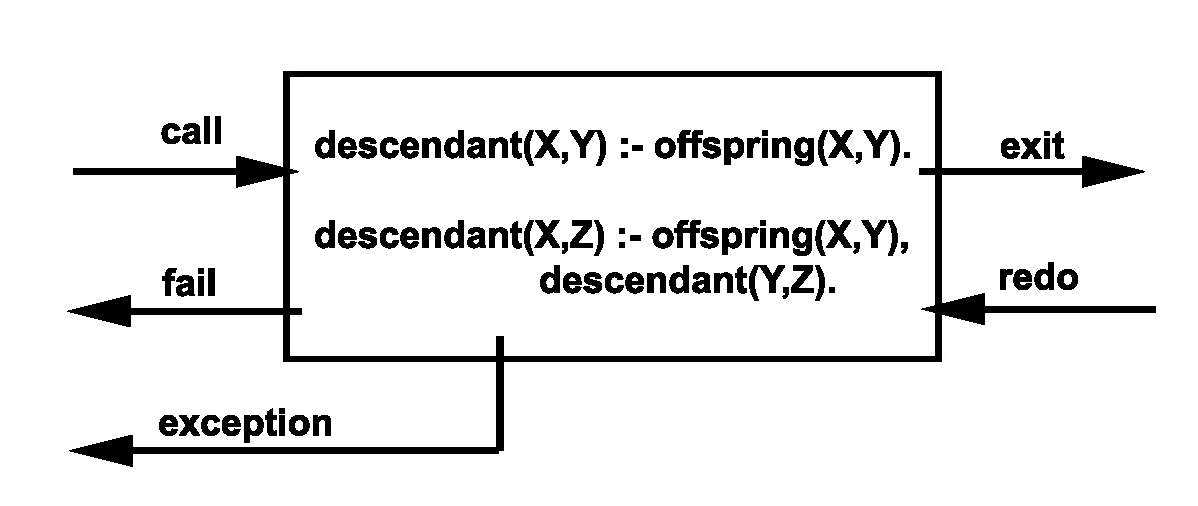
\includegraphics[height=5cm]{images/prolog-debugging.eps}
\end{center}
\end{figure}

SICStus Prolog also provide profiler which can be used to tune program for better 
performance.

Program in SICStus Prolog can be integrated to larger project by using C/C++ interface.
C/C++ programs can call SICStus Prolog code as well as SICStus Prolog can call C/C++
procedures. There also exists interface to Java/.NET which can be called over network.

There is support for graphical output of results as well as defining windows to
interact with users. SICStus Prolog uses for that purpose Tk toolkit. 

SICStus prolog provides lots of built in predicates which can user use to various 
tasks from sorting lists to communicating over network (\cite[chapter 10]{sicstus:manual}).

\section{\eclipse}\label{eclipse}

\subsection{Description}

\eclipse is open source constraint satisfaction solving system based on Prolog 
programming language. The system is based on the Prolog programming
language which is extended with new predicates and operators. Prolog extensions are 
more described in "Modelling Capabilities" subsection. One of \eclipse system goals 
is to be as much compatible with SICStus Prolog as possible. 

\subsection{Modelling capabilities}

Modelling capabilities are almost the same as in SICStus Prolog. There is only few
differences, mostly in naming of predicated or their parameters.

\subsection{Programming support features}

Just like in modelling capabilities also programming support is similar to SICStus
Prolog. 

** NAJIT NEJAKY ROZDIL... LIBOVOLNY ***


\section{Gecode}

\subsection{Short description}

Gecode is C++ CSP library developed at Royal Institute of Technology in Stockholm.
Just like Choco Gecode does not offer whole IDE but only interface which can be 
linked into users application to use it as independent solver. Gecode strongly uses
templating and operator overloading. This fact combined with nonexistence of tutorial
documentation (there exists only doxygen like documentation) makes learning of 
using Gecode difficult. However after further studying of system internal user is
able to use it efficiently. 

\subsection{Modelling capabilities}

Gecode supports all basic constraints and offers ways how to add new ones. Most 
of the constraints are implemented as overloaded operators which -- as stated before --
makes finding apropriate constrain in documentation difficult but once user know
it (or guess it) it is very easy to use.

Typical way how to implement problem starts with declaring of class which 
is inherited from base class {\em Space} with constructor containing definitions of 
variables and constraints. Problem object is then sent to search engine which 
performs search and returns instances of Problem containing solutions.

Following listing shows most important parts of program solving N queens problem.

%\lstset{language=C++}

\lstloadlanguages{C++}

\definecolor{bgcolor}{rgb}{1,1,0.6} % definice barvy

\lstset{         % nastaveni prostredi listings
  language=C++,
	basicstyle=\tiny,
  keywordstyle=\bfseries,
  identifierstyle=\itshape,
  stringstyle=\ttfamily,
  numbers=none,
  numberstyle=\tiny,
  numbersep=5pt,
  frameround=ffff,
  extendedchars=true,
  tab=~,
  tabsize=2,
  frame=single,
  captionpos=b,
  showspaces=false,
  showstringspaces=false,
  breaklines=true
}


\begin{figure}[ht]
\caption{Example of blah blah}
\begin{lstlisting}
class Queens : public Space {
protected:
	IntVarArray q;

public:
	Queens( int n ) : q(this, n, 1, n) {
		
		for (int i = 0; i<n; i++)
			for (int j = i+1; j<n; j++) {
			  post(this, q[i] != q[j]);
			  post(this, q[i]+i != q[j]+j);
			  post(this, q[i]-i != q[j]-j);
			}

		post( this, q[0] < q[n-1] );
		
		branch(this, q, INT_VAR_SIZE_MIN, INT_VAL_MIN);
	}

  Queens(bool share, Queens& s) :  Space(share,s) {
    q.update(this, share, s.q);
  }
  /* ... */
};

int main(int argc, char* argv[]) {
  Queens *q = new Queens(8);
  DFS<Queens> e(q);
  delete q;
  
  while(1) {
	  Queens* ex = e.next();
	  if (ex == NULL)
		break;
	  ex->print(std::cout);
	  delete ex;
  }

  return 0;
}
\end{lstlisting} 
\end{figure}

\section{Choco}

\subsection{Short description}

Choco is java library for solving CSP distributed as jar archive. Therefore it can
be used in every Java program which allows easily integrate CSP solver to applications.
Project is available at Sourceforge where user can found sources, documentation (in 
JavaDoc and wiki system with several tutorials) and binaries (compiled jar archive).

Beacuse Choco is Java library, it does not need its own IDE and compiler. User can
use for example Eclipse IDE or other Java development tools by his preference.

Authors are now developing Choco2 which is going to obsolete Choco but in time of 
writing of this thesis Choco2 is still under development.

\subsection{Modelling capabilities}

Choco can model CSP over finite domain and experimentaly over real domain. All 
constraints are implemented as member functions of Problem class. User can write his
own child class of Problem and in this child class redefine constraints or add some
new constraints which which could better express constraints needed in problem
description.

\section{Mozart}

\subsection{Short description}

Mozart is CSP solver implementing programming language Oz. Oz contains most of the 
concepts of the major programming paradigms, including logic, functional (both 
lazy and eager), imperative, object oriented, constraint, distributed, and 
concurrent programming. In addition to multi paradigm programming, the major 
strengths of Oz are in constraint programming and distributed programming.

Mozart uses as its interface Emacs editor which is customized for oz files. 
User can directly send source to compiler and code is immediately executed.
 

\subsection{Modelling capabilities}

Mozart provides library for finite domain CSP which can user use to solve CSP as 
well as maximization/minimalization task using objective function. User can choose
propagation method - first fail, naive, etc. as well as his own propagation method.
In case of optimising task user can define order function which is used to select
best solution of all.

*** POPSAT VICE ***

\begin{figure}[ht]
\begin{minipage}[t]{5.0cm}
\caption{\label{srq-mozart-folded}Mozart Explorer -- solution of SRQ in folded version}
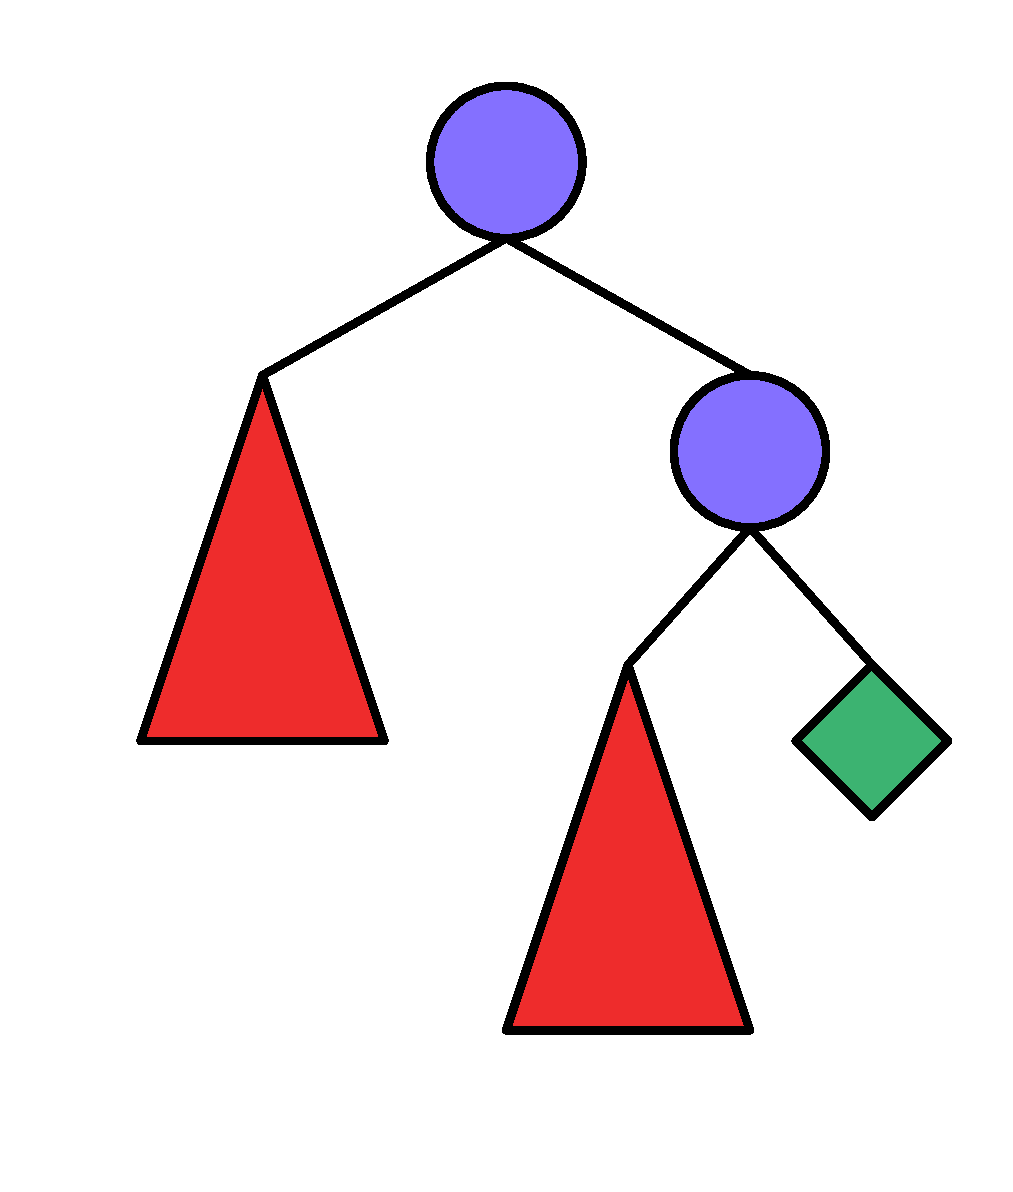
\includegraphics[height=5cm]{images/mozart/srq.oz.color.folded.eps}
\end{minipage}
\hfill
\begin{minipage}[t]{6.0cm}
\caption{\label{srq-mozart-unfolded}Mozart Explorer -- solution of SRQ in unfolded version}
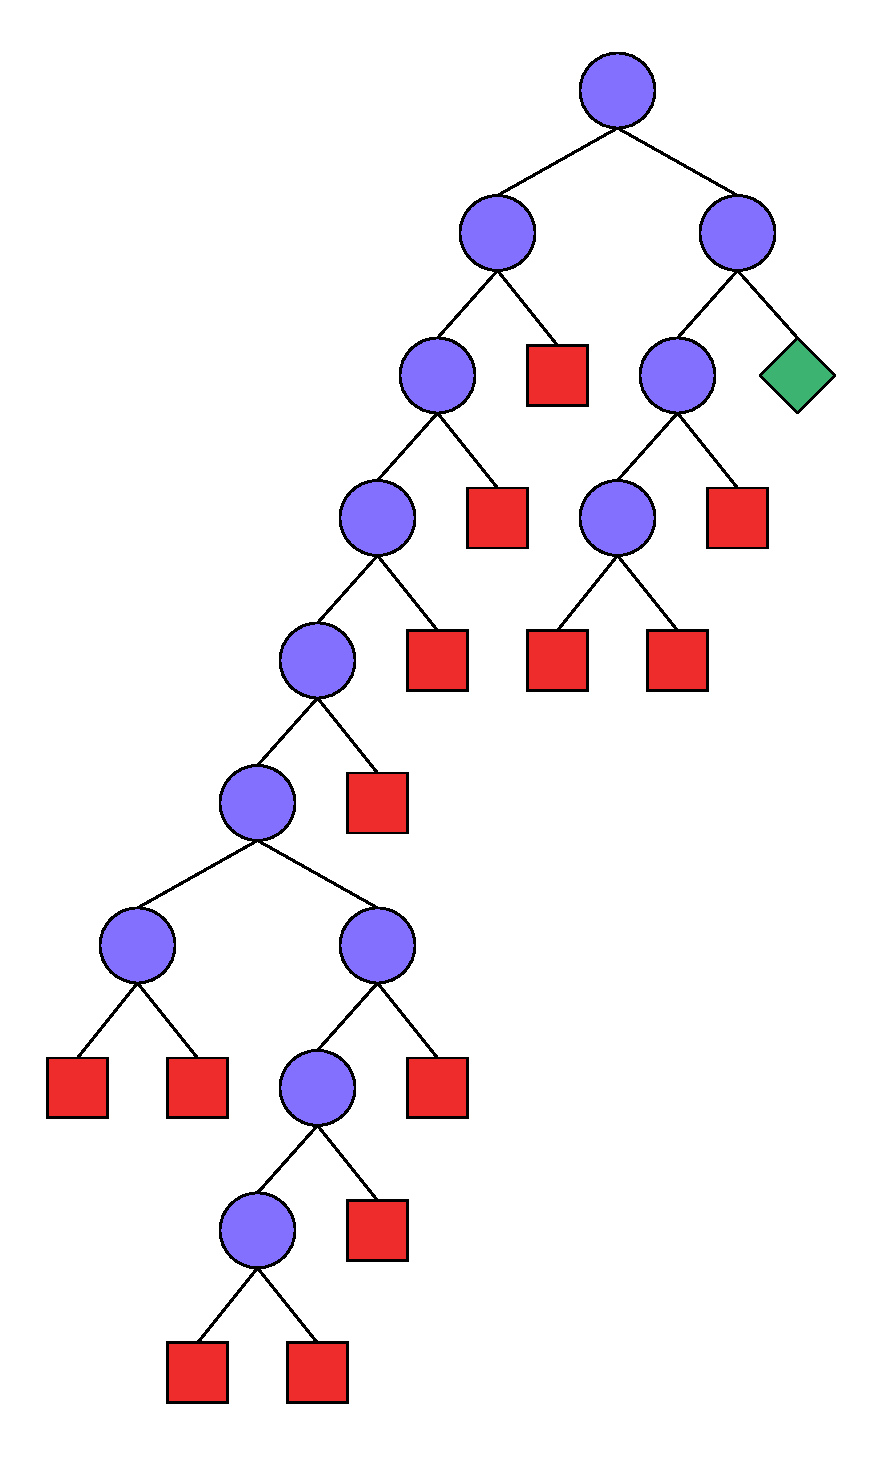
\includegraphics[height=8cm]{images/mozart/srq.oz.color.unfolded.eps}
\end{minipage}
\end{figure}

\subsection{Programming support features}

Mozart provides tool {\em Oz Explorer} (screenshot is in figure 
\ref{mozart-explorer-screenshot}; circle mean choice, square 
"failure - no solution" and diamond means solution). User can browse 
solutions and choices and by double clicking inspect state of variables 
in decision tree nodes. The computing is directed from the explorer. 
By default the solving is stopped after first solution is found. User 
then can inspect results and select partial solutions (nodes which does
not have fully searched all child trees) and start search for next 
solution in that node. 

\begin{figure}[ht]
\caption{\label{mozart-explorer-screenshot}Mozart Explorer}
\begin{center}
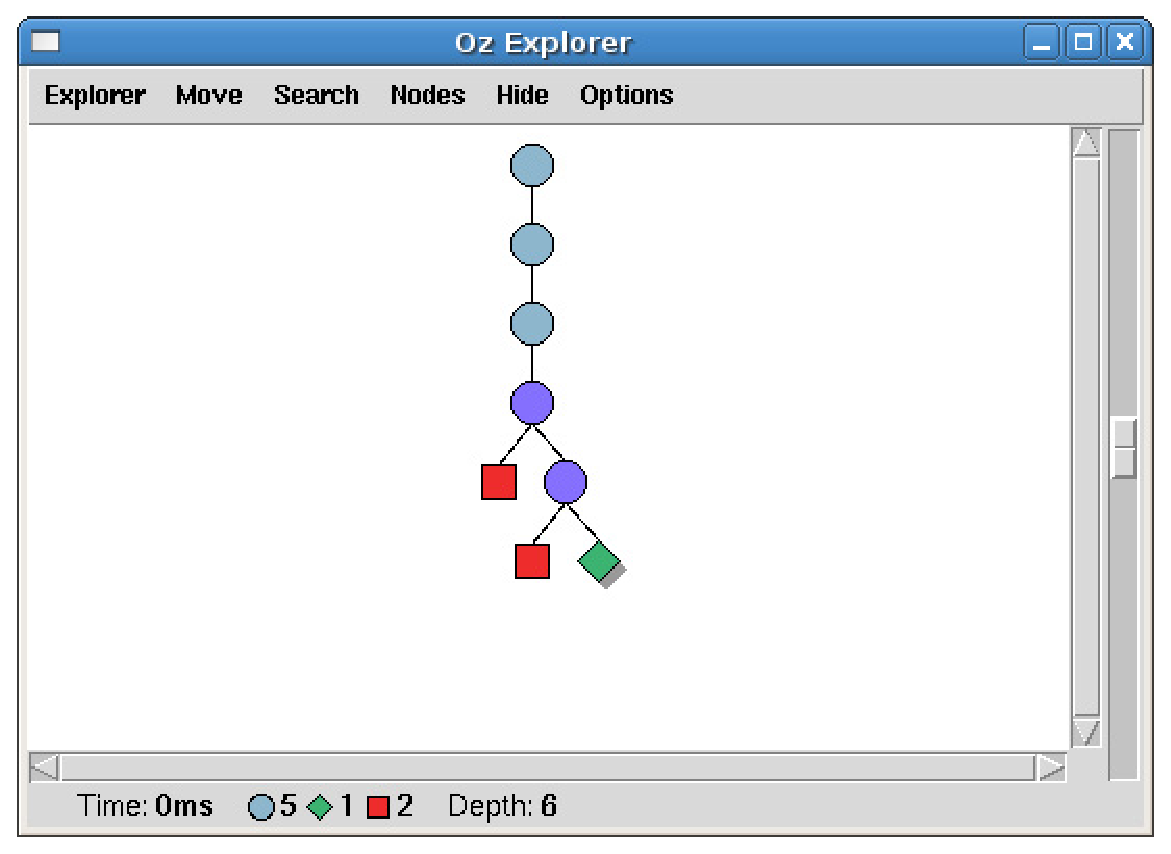
\includegraphics[height=5cm]{images/screenshoty/explorer.eps}
\end{center}
\end{figure}

Another tool provided with mozart is {\em Oz Inspector} (screenshot is in
figure \ref{mozart-inspector-screenshot}). User can call 
it to show messages from the program or to inspect nodes in Oz Explorer.
If the value of inspected variable is updated during inspection the 
showed value alters to correspond with actual value.

\begin{figure}[hb]
\caption{\label{mozart-inspector-screenshot}Mozart Inspector}
\begin{center}
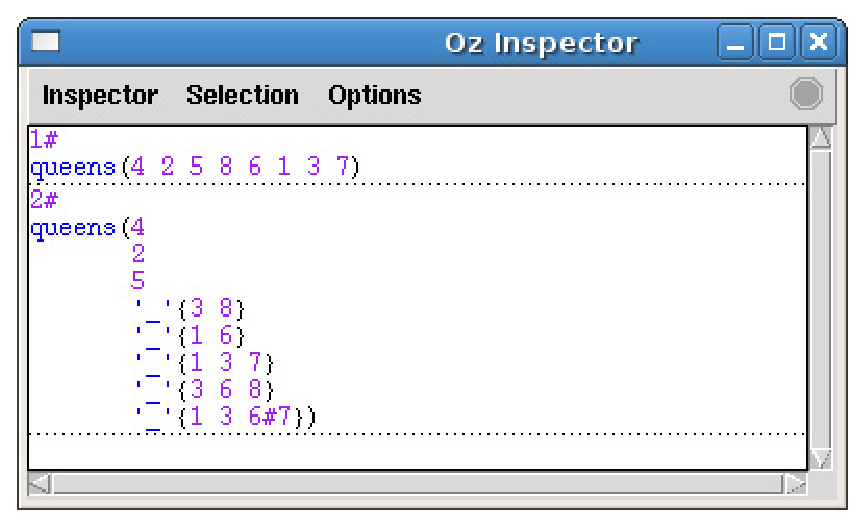
\includegraphics[height=5cm]{images/screenshoty/inspector.eps}
\end{center}
\end{figure}

For debugging Mozart provides tool called {\em Ozcar} where user can step program, 
set breakpoints and perform other actions which can be expected by debugging tool.
Using tool user can inspect call stack and also test immediate input, evaluate 
expression and exec statements. Debugger contains independent utility called
{\em Oz Profiler} which can be used to find nonefficient parts of code and tune 
application for maximal efficiency.

For interaction with its environment Oz provides easy to use ways how to exchange
data with foreign applications. Data can be written to file, sent over network or
sent through pipe to another process.

Mozart provides more features like C/C++ interfacing, distributed programming etc.
More information can be found in \cite{mozart:documentation}.

\section{Minion}

\subsection{Description}

Minion is very low level CSP system with strictly limited set of commands. One 
can describe programming in minion as "constraint satisfaction machine language".
As an example we can demonstrate in on the 4-queens problem.

Common description is:

\begin{align}
\forall i,j, i \neq j & : Q_i \neq Q_j \\
\forall i,j, i < j & : | Q_i - Q_j | \neq j - i 
\end{align}

However in minion there has to be twelve auxiliary variables. Minion does not 
support "sum is equal". If user want to achieve "sum is equal" constraint it has 
to be modified from


Also there is nothing like for or while cycles, whole problem has to be defined in
the input file, which makes programming in pure minion really difficult and nearly
impossible to scale because of growing of auxiliary variables.

The 4-queen problem then looks as follows

\begin{equation*}
\begin{gathered}
Q_2 - Q_3 \leq a_0 \\
Q_1 - Q_3 \leq a_2 \\
Q_1 - Q_2 \leq a_4 \\
Q_0 - Q_3 \leq a_6 \\
Q_0 - Q_2 \leq a_8 \\
Q_0 - Q_1 \leq a_{10}
\end{gathered} \qquad \begin{gathered}
Q_2 - Q_3 \geq a_0 \\
Q_1 - Q_3 \geq a_2 \\
Q_1 - Q_2 \geq a_4 \\
Q_0 - Q_3 \geq a_6 \\
Q_0 - Q_2 \geq a_8 \\
Q_0 - Q_1 \geq a_{10}
\end{gathered} \qquad \begin{gathered}
| a_0 | = a_1 \\
| a_2 | = a_3 \\
| a_4 | = a_5 \\
| a_6 | = a_7 \\
| a_8 | = a_9 \\
| a_{10} | = a_{11}
\end{gathered} \qquad \begin{gathered}
a_{11} \neq 1 \\
a_9 \neq 2 \\
a_7 \neq 3 \\
a_5 \neq 3 \\
a_1 \neq 1 \\
\text{alldifferent}(Q_1,Q_2,Q_3,Q_4)
\end{gathered}
\end{equation*}

As one can see, the problem is described strictly for four queens variant. If there is 
need to extend number of queens whole problem description has to be rewritten.

Fortunately there exists java program Tailor by Andrea Rendl. Tailor converts program
written in Essence' programming language to input format of Minion. Essence' is solver
independent language which describe CSP. More information about this programming language
can be found in \cite{constraints:essence}. Essence' defines syntactic sugar constructions
like \verb=forall= (abbreviation for $a_1 \mand a_2 \mand a_3 \mand \dots$), 
\verb=exists= (abbreviation for $a_1 \mor a_2 \mor a_3 \mor \dots$), \verb=sum= and others.

Great advantage compared to standard Minion input is possibility to scale problems
with given variable. In Minion, the input file can specify for example 4-queens problem 
but for other number of queens is the file unuseful. Programs in Essence' can be written
using constants which are substituted during translation to Minion input format.
As an example of Essence' program we will show 4-queens problem in figure \ref{essence-source-4queens} 
on page \pageref{essence-source-4queens}.  

\begin{figure}[hb]
\caption{\label{essence-source-4queens}Example of 4-queens program in Essence'}
\begin{verbatim}
language ESSENCE' 1.b.a
find queens: matrix indexed by [int(1..n)] of int(1..n)
such that
forall i: int(1..n). forall j: int(i+1..n).
  | queens[i] - queens[j] | != | i - j |,
  alldiff(queens)
letting n to be 4
\end{verbatim}
\end{figure}

During translation Tailor normalize Essence' program then converts it to flat Essence'.
Flat Essence' is program in essence which does not contain any syntactic sugar structures.
This program is then converted to Minion input format.

Tailor is written in Java and is distributed as JAR package. It provides graphic interface
with editor of Essence' code. User can directly convert program in Essence' to Minion
and then run it and see the result if any. Tailor can be also used as non-interactive 
tool which only converts from Essence' to Minion.

\subsection{Modelling capabilities}

Minion can evaluate constrained variables of types {\em bool}, {\em discrete}, {\em bound} 
and {\em sparsebound}. Bool variable has $\{0,1\}$ domain with special 
optimised data structure which provides better performance. Domain of discrete variable is 
range of integers. Memory usage and worst-case performance of most operations
is $O(\text{domain size})$. Discrete domain variable can represent any
subset of domain. Bound variable has domain consisting of range of integer.
In contrast to discrete variable the variable can be only reduced by 
changing one of its bounds. Memory and wors-case performance of all 
operations is $O(1)$   Finally sparsebound variable is identical to 
bound variable with exception that domain is an arbitrary range of 
integers. Further description of variable types and performance of 
their using can be found in \cite{minion-manual}. The variables can
form matrices, vectors and tensors (matrices with more dimensions).
Minion provides acces to whole row/column of matrix using syntax 
\verb=q[5,_]= which means "all values of row 5 of matrix $q$".

Minion does not permit nesting of constraints or array indexes. If user 
needs constraints in form \verb=eq(abs(a),6= he must introduce new auxiliary
variable and declare \verb=abs(a, aux) eq(aux,6)=. Also there is no constraint
stating $\sum{a_i} = b$ and user must declare $\sum{a_i} \leq b$, $\sum{a_i} \geq b$.
These facts makes practical programming in Minion really hard because 
number of auxiliary variables grows very fast. However user still can 
use Tailor to generate input file for Minion.

TODO *** popsat je�t� n�jak� constrainy ***

Result can be simply solution of the CSP or maximation/minimisation of
some given variable.   

\subsection{Programming support features}

Minion is low level black-boxed system which means that there is 
not wide support for user. User can print out log of the 
parsing process. This log contains detailed information about loading 
of variables and could help find problem in the input file. Second 
debugging feature which is built in the minion is possibility of 
printing whole decision tree. This log contains listing of all nodes 
and decisions. Following listing is example of decision tree of 
the 4-queens problem.

{\small
\begin{verbatim}
Node: 0,<{1,2,3,4},{1,2,3,4},{1,2,3,4},{1,2,3,4},{-3,-2,-1,0,1,2,3},
{0,2,3},{-3,-2,-1,0,1,2,3},{0,1,3},{-3,-2,-1,0,1,2,3},{0,2,3},
{-2,-1,0,1,2},{0,1,2},{-3,-2,-1,0,1,2,3},{0,1,3},{-3,-2,-1,0,1,2,3},
{0,2,3}>

Node: 1,<{1,2,3,4},{1,2,3,4},{1,2,3,4},{1,2,3,4},{-3,-2,-1,0,1,2,3},
{0,2,3},{-3,-2,-1,0,1,2,3},{0,1,3},{-3,-2,-1,0,1,2,3},{0,2,3},
{-2,-1,0,1,2},{0,1,2},{-3,-2,-1,0,1,2,3},{0,1,3},{-3,-2,-1,0,1,2,3},
{0,2,3}>

SearchAssign:AnyVarRef:LongRange0 = 1

Node: 2,<1,{3,4},{2,3,4},{2,3},{-1,0,1,2},{0,2},{0,1},{0,1},
{-1,0,1,2},{0,2},{-2,-1},{1,2},{-3,-2,-1},{1,3},{-3,-2},{2,3}>

SearchAssign:AnyVarRef:LongRange1 = 3
SearchAction:bt
SearchAssign:AnyVarRef:LongRange1 != 3
SearchAction:bt
SearchAssign:AnyVarRef:LongRange0 != 1

Node: 3,<{2,3,4},{1,2,3,4},{1,2,3,4},{1,2,3,4},{-3,-2,-1,0,1,2,3},
{0,2,3},{-3,-2,-1,0,1,2,3},{0,1,3},{-3,-2,-1,0,1,2,3},{0,2,3},
{-2,-1,0,1,2},{0,1,2},{-2,-1,0,1,2,3},{0,1,3},{-2,-1,0,1,2,3},
{0,2,3}>

SearchAssign:AnyVarRef:LongRange0 = 2

Node: 4,<2,{1,3,4},{1,3},{1,3,4},{-3,-2,-1,0,1,2},{0,2,3},
{-3,-2,-1,0,1,2,3},{0,1,3},{-2,-1,0,1,2,3},{0,2,3},{-2,-1,0,1},
{0,1,2},{-1,0,1},{0,1},{-2,-1,0,1},
{0,2}>

SearchAssign:AnyVarRef:LongRange1 = 1
SearchAction:bt
SearchAssign:AnyVarRef:LongRange1 != 1

Sol: 2 4 1 3
\end{verbatim}
}

Minion does not offer public include headers and library to use the solver
as CSP subsystem in wider C++ application. However examining of source codes
revealed, that minion sources could be used in such way. *** UVIDIME 
VYSLEDEK DOTAZU NA AUTORY ***.
